\section{Roje dronów}

\begin{frame}{Jak ptaki i owady stają się inspiracją?}
    Zamiast jednego, potężnego drona, z zadaniem lepiej potrafi poradzić sobie rój kilkunastu (lub kilkuset!) małych jednostek. Ale jak uniknąć zderzeń w powietrzu? 
    \vspace{0.3cm}
    
    Opisujemy to matematycznym \textbf{modelem Cuckera-Smale'a}, który opiera się na prostych zasadach:
    \begin{itemize}
        \item \textbf{Separacja}: nie wpadaj na sąsiada.
        \item \textbf{Kohezja}: trzymaj się blisko grupy.
        \item \textbf{Aliniacja (Dopasowanie)}: leć w tym samym kierunku, co reszta.
    \end{itemize}
\end{frame}

\begin{frame}{Rój w środowisku ArduPilot}
    Samo oprogramowanie nie wie początkowo, że ma do czynienia z wieloma maszynami. Zestawiamy architekturę opartą o rozproszoną komunikację między systemami.
    
    \vspace{0.3cm}
    Drony wymieniają się swoim wektorem położenia i prędkości.
    
    \begin{columns}
        \begin{column}{0.5\textwidth}
            \small
            \textbf{Architektura Komunikacji} \\
            Każdy dron wysyła swoją pozycję (GPS) i prędkość przez protokół MAVLink. 
            Algorytm roju odbiera te pakiety, liczy odległości do sąsiadów na podstawie wzorów, i wysyła korekty wektora prędkości.
        \end{column}
        \begin{column}{0.5\textwidth}
            \begin{center}
            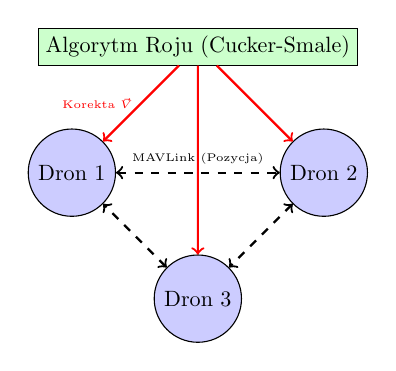
\begin{tikzpicture}[scale=0.8, every node/.style={transform shape}]
                \node (d1) at (0,2) [circle, draw, fill=blue!20] {Dron 1};
                \node (d2) at (4,2) [circle, draw, fill=blue!20] {Dron 2};
                \node (d3) at (2,0) [circle, draw, fill=blue!20] {Dron 3};
                
                \draw[<->, dashed, thick] (d1) -- (d2) node[midway, above, font=\tiny] {MAVLink (Pozycja)};
                \draw[<->, dashed, thick] (d2) -- (d3);
                \draw[<->, dashed, thick] (d3) -- (d1);
                
                \node (algo) at (2,4) [rectangle, draw, fill=green!20] {Algorytm Roju (Cucker-Smale)};
                \draw[->, thick, red] (algo) -- (d1) node[midway, left, font=\tiny] {Korekta $\vec{V}$};
                \draw[->, thick, red] (algo) -- (d2);
                \draw[->, thick, red] (algo) -- (d3);
            \end{tikzpicture}
            \end{center}
        \end{column}
    \end{columns}
\end{frame}

\begin{frame}{Rozdzielenie roju i kontrola odległości}
    W obliczu przeszkody (np. wzniesienie, budynek), ławica musi podjąć decyzję o rozdzieleniu i późniejszym połączeniu.
    
    \vspace{0.3cm}
    Rozwiązując w każdym ułamku sekundy układ równań różniczkowych, drony nieustannie utrzymują zaprogramowany margines odległości (bezpieczeństwa) od innych maszyn.
    
    \begin{columns}
        \begin{column}{0.5\textwidth}
            \small
            \textbf{Omijanie Przeszkód (Boids / Siły Odrzucające)} \\
            Gdy na drodze pojawia się przeszkoda, algorytm generuje wokół niej "pole siłowe" (odpychające). 
            Drony reagują na tę wirtualną siłę rozdzielając się na dwie grupy. 
            Gdy przeszkoda znika, siły kohezji (przyciągania) ponownie łączą rój w jedną ławicę.
        \end{column}
        \begin{column}{0.5\textwidth}
            \begin{center}
            \begin{tikzpicture}[scale=0.8]
                % Przeszkoda
                \node (obs) at (2.5,2.5) [circle, draw, fill=red!40, minimum size=1.2cm] {O};
                \draw[red, dashed, thick] (2.5,2.5) circle (1.2cm);
                
                % Drony omijajace
                \node (d1) at (0,1) [circle, fill=blue, inner sep=1.5pt] {};
                \draw[->, thick, blue] (d1) to[out=45, in=180] (1.5, 3.5) to[out=0, in=135] (4, 2.5);
                
                \node (d2) at (0,4) [circle, fill=blue, inner sep=1.5pt] {};
                \draw[->, thick, blue] (d2) to[out=-45, in=180] (1.5, 1.5) to[out=0, in=-135] (4, 2.5);
                
                \node (d3) at (4,2.5) [circle, fill=green, inner sep=1.5pt] {};
                \draw[->, thick, green] (d3) -- (5,2.5) node[right, font=\tiny] {Połączony rój};
                
            \end{tikzpicture}
            \end{center}
        \end{column}
    \end{columns}
\end{frame}
